\section{Evaluation der Methode an Beispielen}

In diesem Kapitel soll die Anwendbarkeit und Wirksamkeit von \ac{MFEM} untersucht werden. Hierzu wird die Methode an 2 Beispielen durchgeführt und ausgewertet. Es werden sämtliche Phase exemplarisch durchlaufen und dokumentiert. Zudem wird für die Durchführung der 2 Beispiele der Zeitaufwand gemessen, um auch eine Aussage über die Anwendungsdauer zu treffen. Diese spielt eine Rolle für die Akzeptanz der Methode, da eine lange Laufzeit dem Nutzen entgegensteht.\\ 
Als Ergebnis der Evaluation wird sich zeigen, ob die Methode möglichst viele Seiten eines Frameworks betrachtet und dabei repräsentative Resultate liefert.  
Um dies zu gewährleisten, müssen die richtigen Kandidaten gewählt werden.

\subsection{Wahl der Kandidaten}

Um mit der Evaluation von \ac{MFEM} möglichst vertretbare Ergebnisse zu erhalten, wurden folgenden Anforderungen an die Wahl der Kandidaten gestellt:

\begin{description}
	\item[Heterogenität] Da \ac{MFEM} eine sprachunabhängige Bewertungsmethode ist, sollten die Programmiersprachen andersartig sein.
	\item[Diskrepanz] Um Unterschiede in einzelnen Aspekten zu erhalten, sollte der Reifegrad bzw. Entwicklungsstand auseinandergehen.
	\item[Popularität] Die Frameworks sollten aktuell und relevant sein.
	\item[Opportunität] Der Zweck sollte nachgewiesenermaßen für den Einsatz in einer Microservice Architektur sein.
\end{description}

Diesen Anforderungen folgend wurde als Erstes das auf Java basierende Spring Framework\footnote{\url{spring.io}} gewählt. Es befindet sich seit 2002 in Entwicklung und hat seit dem mehrere Preise gewonnen\cite[1]{Gutierrez2016}. Dabei entwickelt es die sehr aktive Open-Source-Community ständig weiter und integriert die neuesten Technologien. Beispiele hierfür sind WebFlux, welches reaktive Webapplikationen ermöglicht, oder Cloud-Contract, um die \ac{REST}-Schnittstelle mit einem Consumer-Driven Contract abzusichern. Zudem findet jährlich die SpringOne Konferenz statt, welche mit über 2000 Teilnehmern und 30 großen Sponsoren für den Erfolg von Spring sprechen\cite{SpringOne2016}.\\
2014 wurde die Erweiterung Spring Boot offiziell veröffentlicht und stellte eine große Evolution des Frameworks dar. Es nimmt dem Entwickler so viel Arbeit wie möglich ab, sodass dieser sich auf die Geschäftslogik konzentrieren kann. Dabei stellt es die Konvention über die Konfiguration und erstellt so automatisch robuste, erweiterbare und skalierbare Spring Applikationen\cite[1]{Gutierrez2016}. Dies spricht für den hohen Reifegrad und die Akzeptanz des Frameworks.\\
Nach \cite{Wolff2016} ist das Spring Framework eine sehr gute Wahl für den Einsatz in einer Microservice Architektur und lässt dabei kaum ein Problem offen, für das es keine Lösung vorhält. 

Die Wahl des zweiten Frameworks fiel auf Go-Kit\footnote{\url{gokit.io}}. Es wird seit 2016 entwickelt und ist somit, im Gegensatz zu Spring, ein sehr junges Framework. Dabei setzen die Entwickler auf die Programmiersprache Go, welche selbst noch relativ jung ist. \\
Go wurde ursprünglich 2007 von Mitarbeitern des Unternehmens Google\cite{Golang2009} entwickelt und ist seit 2012 in einer stabilen Version verfügbar. Seit dem ist das Interesse für diese Sprache immens gestiegen, was der Tiobe Index deutlich zeigt. Dies ist ein Popularitäts-Ranking von Programmiersprachen, in dem Go bereits Platz 14 (Stand: Februar 2017) einnimmt\cite{Tiobe2016}. Aufgrund der starken Steigerung gegenüber dem Vorjahr wurde Go von Tiobe auch zur Programmiersprache 2016 gewählt.\\
Da Go bereits im Hinblick auf skalierbare Netzwerkdienste, Cluster- und Cloud Computing entwickelt wurde, bringt die Sprache bereits sehr viel für die Erstellung von verteilten Systemen mit. In Bezug auf eine Microservice Architektur fehlen jedoch einige Funktionen wie z.~B. Infrastrukturintegration oder Logging. Diese Lücke versucht Go-Kit zu schließen, damit der Entwickler sich auf die Geschäftslogik konzentrieren kann.

Mit Spring und Go-Kit für die Evaluation von \ac{MFEM} werden die Anforderungen nach Heterogenität, Diskrepanz, Popularität und Opportunität erfüllt. Neben den unterschiedlichen Programmiersprachen geht der Reifegrad der Frameworks stark auseinander und sollte somit für unterschiedliche Ergebnisse sorgen. Nichtsdestotrotz erfahren 
beide aktuell einen hohen Zuspruch für den Einsatz in einer Microservice Architektur und stellen somit interessante Kandidaten dar.

\subsection{Kickoff-Phase}

Neben der Einführung der Methode sieht diese Phase eine Vorstellung der vorhandenen Microservice Architektur vor.  
Da ein Teil der Evaluation auf den in \ac{MFEM} enthaltenen Basisanforderungen und deren Wirkung liegen soll, wurde ein möglichst einfacher Entwurf der zugrundeliegenden Architektur gewählt. So ergeben sich in der Analysephase nur wenige spezifische Anforderungen, die für die Evaluation der Methode nur eine geringe Rolle spielen. Weitere Phasen sind von der Microservice Architektur nicht direkt betroffen und bleiben daher unberührt. Abbildung \ref{Evaluationsarchitektur} zeigt die gewählte Architektur.

\image[Evaluationsarchitektur.pdf]{Evaluationsarchitektur}{Architektur für die Evaluation}{Vorgegebene Microservice Architektur für die Evaluation}

Die Architektur teilt sich in Infrastruktur und Services auf. Services enthalten die Ge\-schäfts\-logik sowie Datenhaltung. Dabei kann es verschiedene Services geben, die in mehrere Instanzen vorhanden sein können. Die genaue Form ist für die Evaluation irrelevant und wird daher nicht weiter berücksichtigt. Des Weiteren kümmert sich die Infrastruktur um den reibungslosen Ablauf und ist in Service-Discovery, Authentication-Service und API-Gateway aufgeteilt.

Das API-Gateway stellt eine einheitliche Schnittstelle des Gesamtsystems den Clients zur Verfügung. So müssen diese keine Kenntnis über die interne Struktur haben und können sämtliche Funktionen über einen zentralen Punkt nutzen. Hierzu reicht es die externen Anfragen an die jeweiligen Services weiter.

Die Service-Discovery sorgt für die Verwaltung der einzelnen Services und deren Instanzen, damit diese von anderen, z.~B. dem API-Gateway, erreicht werden können. Jede Instanz eines Services muss sich an der Discovery beim Start registrieren und einen regelmäßigen Heartbeat an diese senden. Hierzu bietet die mit Netflix Eureka erstellte Discovery eine \ac{REST}-Schnittstelle zur Verfügung. Der genaue Ablauf ist in Abbildung \ref{ServiceDiscovery} dargestellt.

\image[ServiceDiscovery.pdf][width=0.5\linewidth]{ServiceDiscovery}{Ablauf Service Discovery}{Ablauf: Zugriff über die Service Discovery}

Der Authentication Service kümmert sich um die Authentifizierung der Benutzer. Damit müssen die einzelnen Services keine eigene Benutzerverwaltung integrieren. Mit der Authentifizierung erhält der Client einen begrenzt gültigen \ac{JWT}, mit dem er auf die Services zugreifen kann. So lassen sich auch kaskadierte Anfragen realisieren, bei dem ein Service mittels des \ac{JWT} einen anderen aufruft ohne die Anmeldeinformationen des Clients zu kennen. Dies ist auch vereinfacht in Abbildung \ref{AuthFlow} dargestellt, wobei die Zwischenschritte über das API-Gateway und die Service-Discovery vernachlässigt wurden.

\image[AuthFlow.pdf][width=0.7\linewidth]{AuthFlow}{Ablauf kaskadierter Anfrage}{Vereinfachte Darstellung einer kaskadierten Anfrage eines Clients über mehrere Services}

Weitere Vorgaben über die Architektur werden nicht gemacht, da diese im Sinne der Evaluation nicht zielführend wären. Wie eingangs geschildert, würde sich dies nur in zusätzlichen Anforderungen widerspiegeln.

\subsection{Analysephase}

In der Analysephase sollen nun mit Hilfe der gegebenen Architektur die Anforderungen gewählt, priorisiert und um Metriken erweitert werden. Hierzu wird im nächsten Schritt ein Quality Utility Tree aufgebaut.

\subsubsection{Architektur Analyse und Wahl der Anforderungen}

Mit \ac{MFEM} kommen bereits viele Anforderungen, die Basisanforderungen, mit. Da die Architektur möglichst einfach gehalten wurde, gibt es keinen Widerspruch zu diesen Anforderungen. Sie lassen sich somit vollständig übernehmen.

Zusätzlich ergeben sich aus der Architektur funktionale Serviceanforderungen. Dies betrifft hauptsächlich die Service-Discovery. Ein Service muss sich an diesem An- und Abmelden sowie regelmäßig einen Heartbeat senden. Auch für die Inter-Service-Kommunikation muss ein Service an der Discovery die Einträge abfragen und verarbeiten können. (Abbildung \ref{ServiceDiscovery}) Somit wurde die Anforderung zur Unterstützung einer mit Eureka aufgebauten Service-Discovery aufgenommen.

In den Basisanforderungen ist bereits unter der Kategorie Sicherheit die Anforderung nach einer Absicherung gefordert. Dies beinhaltet die Unterstützung eines \ac{JWT} und wird daher nicht als eigener Punkt aufgenommen. Zusätzlich soll auf eine Autorisierung durch Benutzer zugehörige Rechte verzichtet werden. 
Aus diesem Grund ergeben sich durch den Authentifizierungs-Service keine weiteren Anforderungen.\\
Auch durch das Gateway ergeben sich keine Anforderungen, da die Beziehung zu den Services einseitig ist. Im vorliegenden Entwurf leitet das API-Gateway Anfragen an die Services weiter. Jedoch stellen die Services keine Anfragen an das Gateway und müssen daher keine zugehörigen Funktionen unterstützen.

Die Basisanforderungen decken bereits eine Vielzahl an nicht-funktionalen Serviceanforderungen ab. Diese beinhalten z.~B. die Forderung nach einer aktiven Community, eine effiziente Programmierung oder eine gute Dokumentation. Aus diesem Grund wird auch hier auf die Aufnahme weiterer Anforderungen verzichtet.

Nachdem alle Anforderungen zusammengetragen und in einem Quality Utility Tree eingeordnet wurden, sind diese Priorisiert worden. Abbildung \ref{QUT} zeigt den entstandenen Quality Utility Tree mit allen Anforderungen für die Evaluation.

\image[QUT.pdf][width=0.7\linewidth]{QUT}{Quality Utility Tree Evaluation}{Priorisierter Quality Utility Tree mit allen Anforderungen für die Evaluation.}

\subsubsection{Metriken definieren}

Mit dem Ergebnis aus dem letzten Schritt können nun die passenden Metriken für die Anforderungen gefunden werden. \ac{MFEM} sieht hierfür den Top-Down Ansatz der \ac{GQM} Methode vor.\\
Das heißt, dass für jede Anforderungen eine oder mehrere Fragen erstellt werden, die zusammen das Ziel wiedergeben. Sie drücken somit aus, was man mit der Messung erfahren will und betrachten die Anforderung von mehreren Seiten.\\
Für alle Anforderungen wurden so Fragen erstellt und in einer Tabelle festgehalten. Darauf aufbauend wurden Metriken definiert, die die Fragen beantworten sollen.

Die gesamte in diesem Schritt erstellte Tabelle wird in \ref{GQM} dargestellt und enthält das Ergebnis der Anwendung von \ac{GQM} auf die Anforderungen mit allen definierten Metriken.  

\begin{longtable}{c}
	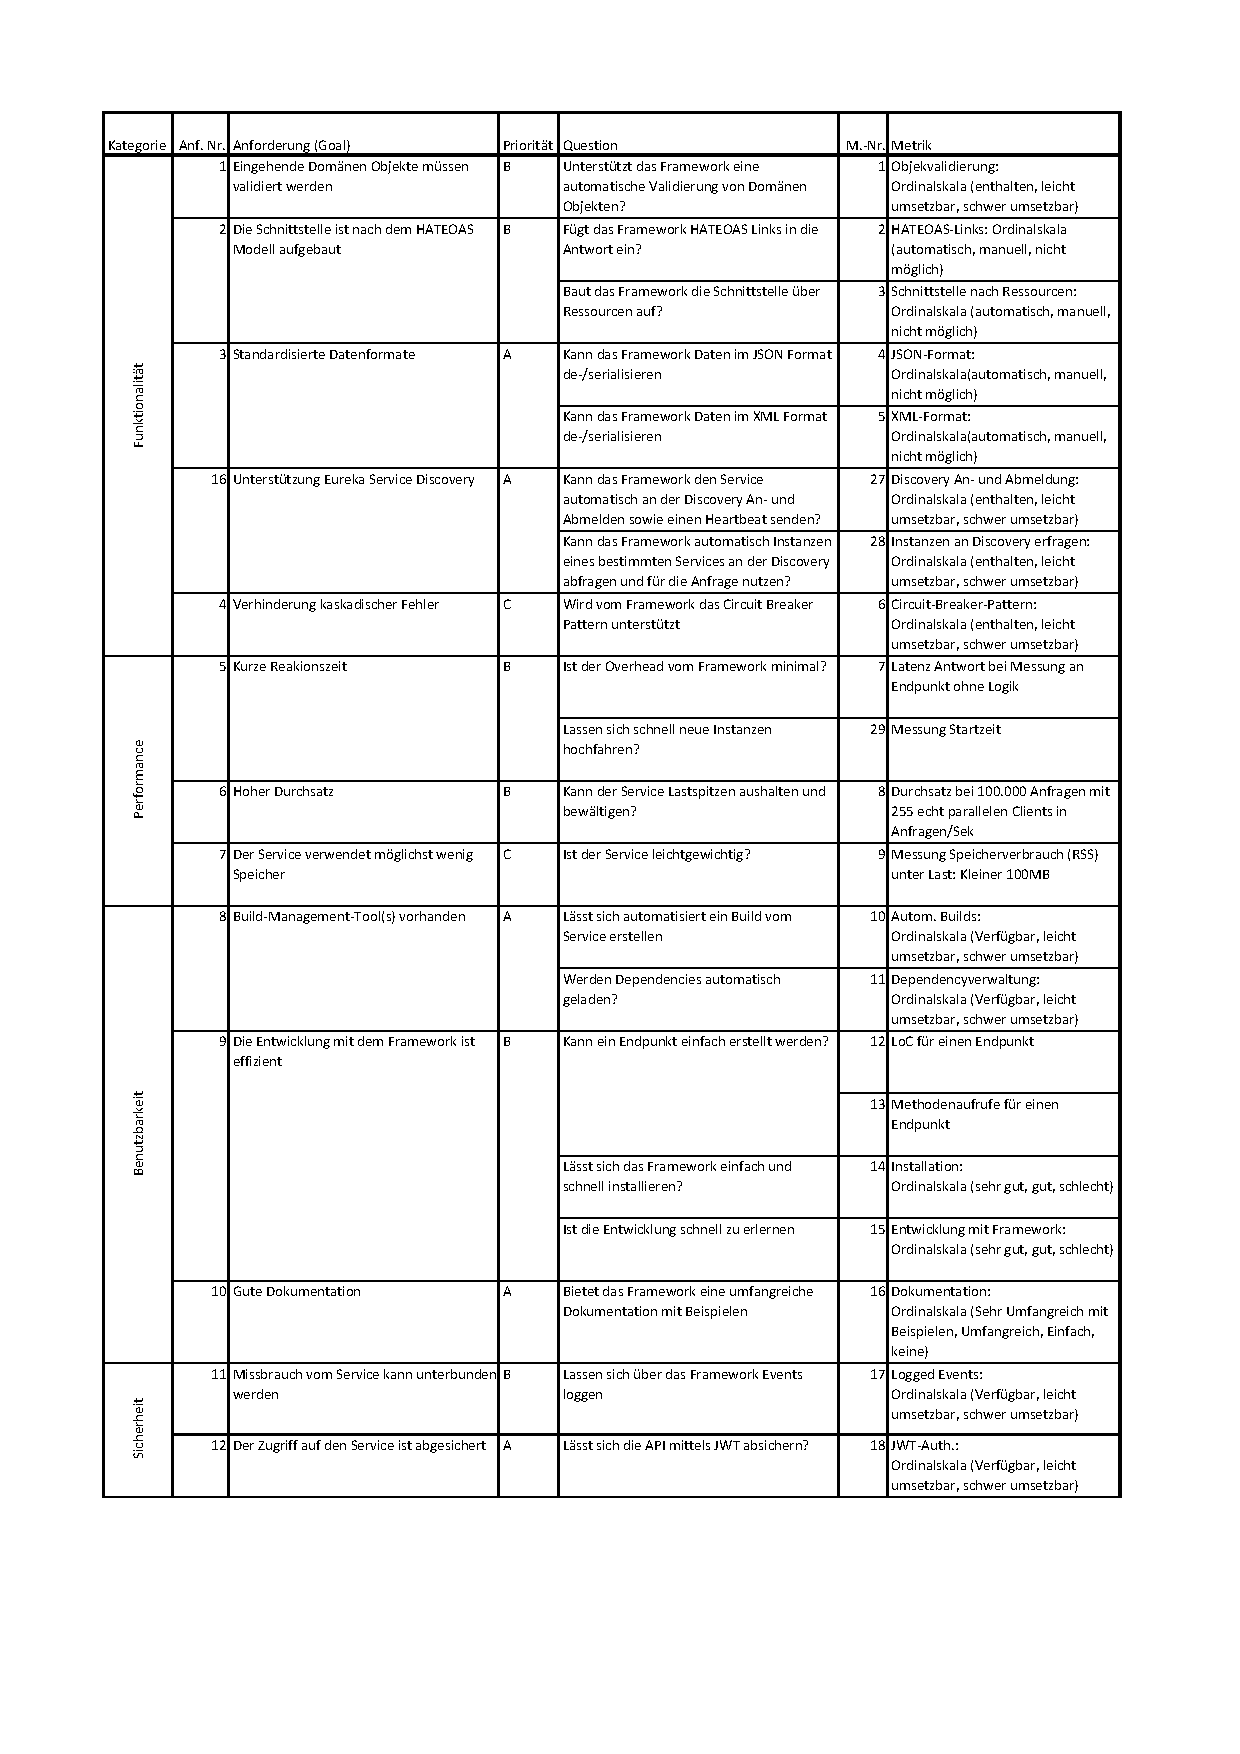
\includegraphics[width=\linewidth]{Bilder/GQM.pdf} \\	
	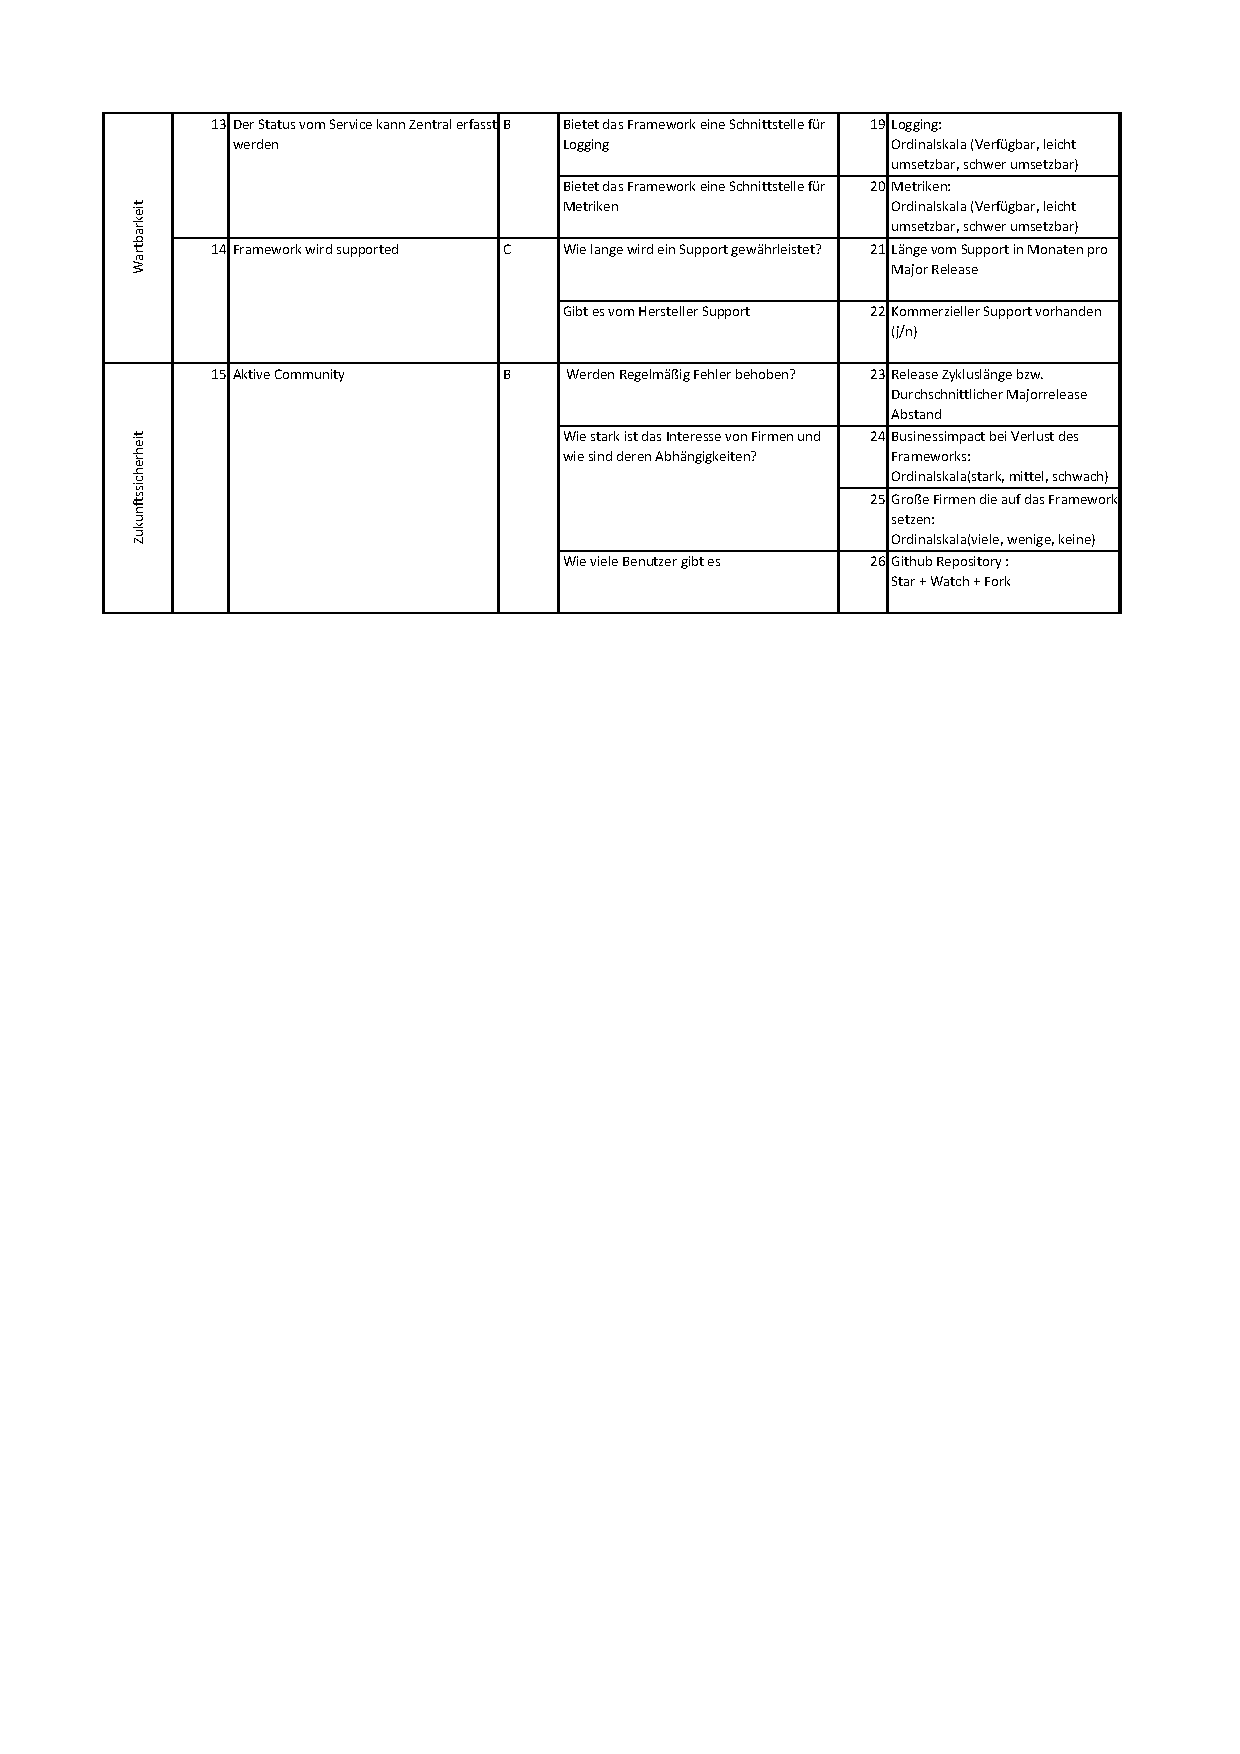
\includegraphics[width=\linewidth]{Bilder/GQM2.pdf}	\\
	\caption[Evaluation: Goal Question Metrik Tabelle]{Goal Question Metrik Ergebnis als Tabelle dargestellt}
	\label{GQM}\\
\end{longtable}
\FloatBarrier

\subsection{Evaluationsphase}

In der Evaluationsphase wird nun der Ablauf der Evaluation geplant und durchgeführt. Hierzu werden im nächsten Schritt Szenarien definiert.

\subsubsection{Evaluation definieren}

Die Evaluation wird in subjektiv und objektiv aufgeteilt. Für die subjektive Evaluation werden Szenarien definiert, die die Anforderungen bzw. Metriken untersuchen sollen.\\
\ac{MFEM} sieht hierzu die Definition eines Standard-Anwendungsfalls vor, der in mehrere Teile, den Szenarien, aufgeteilt wird. Hier wurde die Erstellung eines einfachen Daten-Service definiert, der sich mit dem Beispiel aus Kapitel \ref{Evaluation_definieren} deckt. Aus diesem Grund werden auch die Beispiel-Szenarien aus Kapitel \ref{Evaluation_definieren} übernommen und hier nur nochmal kurz zusammengefasst:

\begin{description}[leftmargin=!,labelwidth=\widthof{\bfseries Sz.3 Erweiterter Service}]
	\item[Sz.1 Installation] Installation der Sprache sowie des Frameworks und Einrichtung der Build-Tools
	\item[Sz.2 Einfacher Service] Programmierung eines einfachen "Hello World"-Services, inklusive Security
	\item[Sz.3 Erweiterter Service] Erweiterung des einfachen Services um ein Datenmodell (Aufgabenverwaltung)  
\end{description} 

Für die objektive Evaluation stehen nach \ac{MFEM} bereits Messgruppen fest. Diese umfassen die Messung an Artefakten, wie z.~B. dem Code, die Performance-Messung am lauffähigen Prototyp sowie der Recherche.\\
Um für die Messungen am laufenden Prototyp definierte Umstände zu haben, werden hier noch Anforderungsprofile benötigt. Dabei wurden folgende Profile für die Evaluation festgehalten:

\begin{table}[!h]
	\centering
	\begin{tabular}{p{1cm}p{4cm}p{2cm}p{2cm}p{4cm}}
		\textbf{Nr.} & \textbf{Typ} & \textbf{Parallele Verbindungen} & 
		\textbf{Dauer} & \textbf{Besonderheit} \\
		\hline
		1 	& Datenservice 			& 255	&	30s		& CRUD Operationen auf Datenbank  \\
		\hline
		2	& Einfacher Service		& 255 	&	30s		& Wenig rechenintensive Geschäftslogik   \\
		\hline
	\end{tabular}
	\caption[Anforderungsprofile]{Anforderungsprofile für die objektiven Evaluation am Prototyp}
	\label{AnforderungsprofileEval}
\end{table}

Insgesamt ergeben sich für den nächsten Schritt somit 6 Messgruppen, denen Metriken zugeordnet werden können.
Diese sind in Abbildung \ref{MessgruppenEval} nochmal zusammengefasst.

\image[MessgruppenEval.pdf]{MessgruppenEval}{Messgruppen für Evaluation}{Zusammenfassung aller Messgruppen für Evaluation}

\subsubsection{Metriken zuordnen}



\subsubsection{Evaluation durchführen: Spring Boot}



\subsubsection{Evaluation durchführen: Go-Kit}



\subsection{Abschlussphase}



\subsection{Methodenauswertung}




